\section{Frequency-domain filtering: ideal, Butterworth, Gaussian}

Everything in this problem goes through the zero-padded pipeline from 1.3
\cite{gonzalez}. I pad the image with zeros at the bottom and right to
$P\times P$ with $P=2N$, centre the spectrum with \code{fftshift}, multiply by a
real zero-phase $H(u,v)$, invert, keep the real part and crop. For the two
non-square images (\code{text\_gaps} is $444\times508$, \code{thumb\_print} is
$962\times1026$) I use a square grid with $P=2\max(\text{rows},\text{cols})$,
so that a given $D(u,v)$ means the same frequency along both axes. A distance
$D$ in frequency bins is $D/P$ cycles per pixel. The step image $s(x,y)$ is a
$256\times256$ square of value $B=200$ on a background $A=50$, covering rows and
columns 128 to 383.

\subsection{Filter construction and transfer functions}

\code{make\_filter(kind, P, D0, n=None, highpass=False)} in
\code{src/problem\_2/filters.py} has the interface the handout asks for. It
builds $D(u,v)=\sqrt{(u-P/2)^2+(v-P/2)^2}$ and then one of
\begin{equation}
H_\text{ILPF}=\begin{cases}1&D\le D_0\\0&D>D_0\end{cases},\qquad
H_\text{BLPF}=\frac{1}{1+(D/D_0)^{2n}},\qquad
H_\text{GLPF}=e^{-D^2/2D_0^2},\qquad H_\text{HP}=1-H_\text{LP}.
\end{equation}
Fig.~\ref{fig:tf} plots all six on one axis.

\begin{figure}[H]
\centering
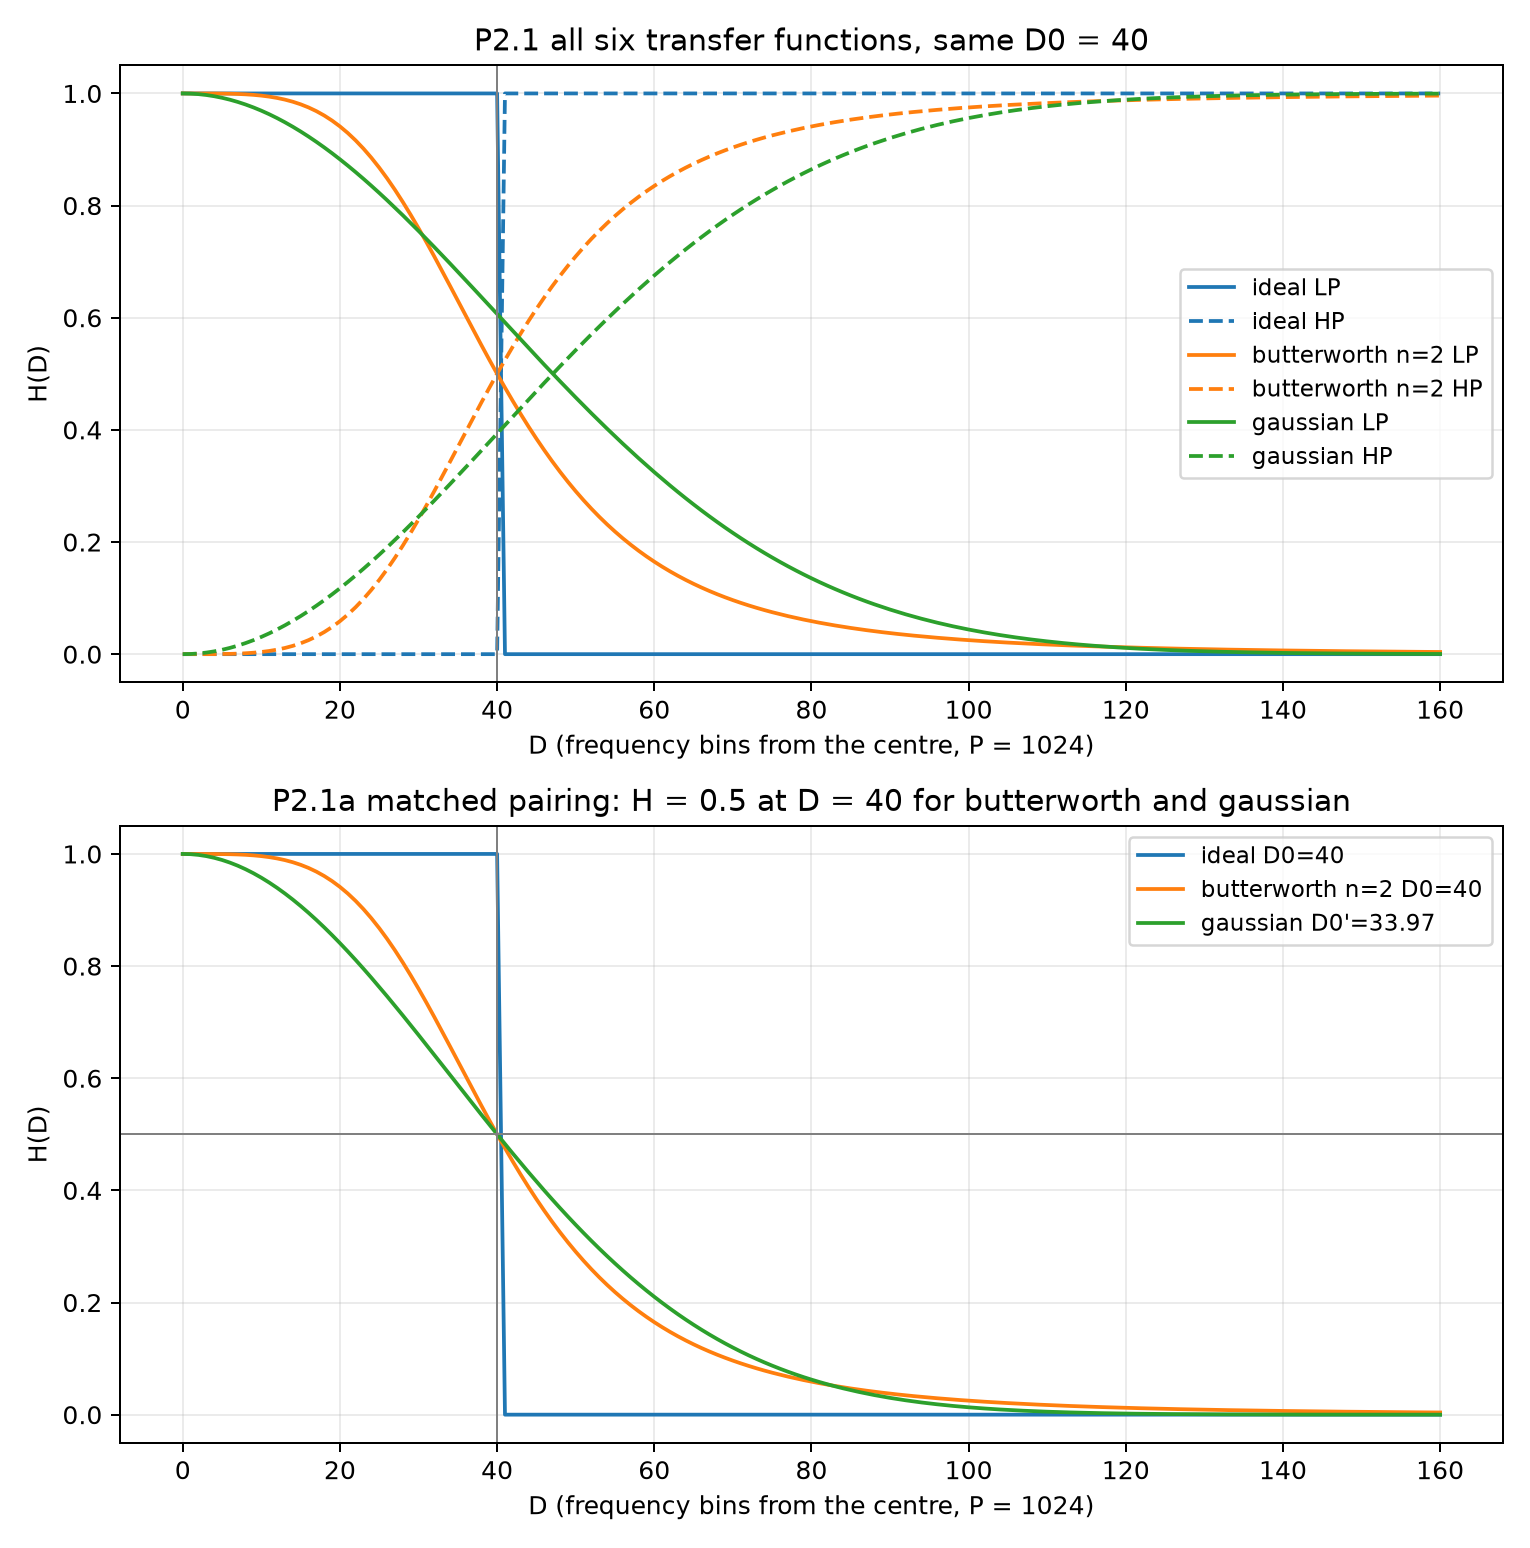
\includegraphics[width=0.95\linewidth]{problem_2/transfer_functions.png}
\caption{Left: the six transfer functions against $D$ (frequency bins from the
centre) for the same $D_0=40$ with $P=1024$ and Butterworth $n=2$. Right: the
matched pairing used in every later comparison.}
\label{fig:tf}
\end{figure}

\paragraph{(a) Cutoff semantics.} Putting $D=D_0$ into each formula gives
$H_\text{ILPF}=1$ (the definition includes $D=D_0$), $H_\text{BLPF}=1/(1+1)=1/2$
for every order, and $H_\text{GLPF}=e^{-1/2}=0.606531$. \code{make\_filter}
returns exactly these values (\code{cutoff\_semantics.txt}). So the same number
$D_0$ means three different things: the last frequency the ideal filter passes,
the half-amplitude point of the Butterworth filter, and the one standard
deviation point of the Gaussian. Comparing them at equal $D_0$ is therefore not
fair. To put the Gaussian's half-amplitude point at the Butterworth cutoff
$D_0$, I solve
\begin{equation}
e^{-D_0^2/2D_0'^2}=\tfrac12\;\Longrightarrow\;\frac{D_0^2}{2D_0'^2}=\ln2\;\Longrightarrow\;
D_0'=\frac{D_0}{\sqrt{2\ln2}}=\frac{D_0}{1.177410}.
\end{equation}
For $D_0=40$ this gives $D_0'=33.9729$, and the built filter has $H=0.500000$
at $D=40$. \textbf{From here on, every Gaussian is described by its
half-amplitude radius $D_0$ and built with $D_0'$.}

\paragraph{(b) Energy-based cutoff.} For the characters pattern padded to
$P=1376$ I computed $\alpha(r)$ by sorting all bins by $D$ and accumulating
$|F|^2$.

\begin{table}[H]
\centering
\begin{tabular}{rrr}
\toprule
target $\alpha$ & radius $r$ (bins) & $\alpha(r)$\\
\midrule
90\,\% & 15.30 & 90.0033\,\%\\
95\,\% & 45.54 & 95.0002\,\%\\
99\,\% & 409.04 & 99.0000\,\%\\
99.5\,\% & 558.74 & 99.5000\,\%\\
\bottomrule
\end{tabular}
\caption{Radii that enclose a given share of the spectral power, characters
pattern, $P=1376$ (\code{power\_retention.txt}, curve in
\code{power\_retention.png}).}
\label{tab:power}
\end{table}

The DC bin alone holds 22.4\,\% of the power and radius 5 already holds
81.6\,\%. The pattern is mostly a flat light background with mean 207, and the
zero padding turns the whole image into one big bright rectangle, so most of the
power just describes the mean level and the outline of that rectangle. Edges put
a small amount of power into a very large number of high frequencies: the last
5\,\% of the power lies beyond $r=45.5$ and the last 1\,\% beyond $r=409$. Those
frequencies are what we actually see, though. They carry the position and
sharpness of every stroke and bar, and the eye cares much more about edges than
about the little power they hold. Fig.~\ref{fig:grid} shows that keeping 95\,\%
of the power still leaves the text badly blurred.

\paragraph{(c) Inverse design.} From $H(10)=16/17$,
\[
1+\Big(\frac{10}{D_0}\Big)^{2n}=\frac{17}{16}\;\Longrightarrow\;\Big(\frac{10}{D_0}\Big)^{2n}=\frac1{16},
\]
and from $H(40)=1/17$, $(40/D_0)^{2n}=16$. Dividing the second by the first
removes $D_0$:
\[
\Big(\frac{40}{10}\Big)^{2n}=4^{2n}=\frac{16}{1/16}=256=4^4\;\Longrightarrow\;n=2.
\]
Then $(10/D_0)^4=1/16$ gives $10/D_0=1/2$, so $D_0=20$. For at most 1\,\% at
$D=2D_0$ I need
\[
\frac{1}{1+2^{2n}}\le0.01\;\Longrightarrow\;4^n\ge99\;\Longrightarrow\;n\ge\frac{\ln99}{\ln4}=3.3147,
\]
so the smallest integer order is $n=4$. As a check,
\code{make\_filter("butterworth", 256, 20, n=2)} gives $H(10)=0.941176=16/17$
and $H(40)=0.058824=1/17$, and $H(2D_0)$ is
$0.200000, 0.058824, 0.015385, 0.003891$ for $n=1,2,3,4$: order 3 misses the
1\,\% target and order 4 meets it (\code{inverse\_design.txt}).

\subsection{Ringing: prediction, measurement and reconciliation}

\textbf{The prediction.} I wrote it on 23 October 2026 at 16:29 IST and
committed it at 16:29 (\code{3c9e956}). Its first line first said 16:31 by
mistake, and I corrected that line eight seconds later in \code{4acb1a0}. No code
had been committed at that point: the first code commit, with the shared FFT
helpers, is at 16:36 (\code{f6ef560}), and the Problem 2 filters and experiments
followed at 16:45 (\code{3618251}, \code{d801bfd}). The full text is
in Appendix~\ref{app:pred-ringing} and in
\code{docs/predictions/p2\_2\_ringing\_prediction.pdf}. The derivation goes as
follows.

Near the middle row and away from the corners, the image looks like a function
of $x$ only, $s(x,y)\approx g(x)$. The DFT of such an image is non-zero only on
the line $v=0$, because the sum over $y$ of $e^{-j2\pi vy/P}$ vanishes for every
$v\ne0$. The filter therefore acts only through its slice $H(u,0)$, and the
filtered row is the 1-D convolution of $g$ with $h(x)=\mathcal F^{-1}\{H(u,0)\}$.
For the ideal filter the slice is a box of half-width $f_c=D_0/P$ cycles/pixel,
so in the continuous model $h(x)=\sin(2\pi f_cx)/(\pi x)$. A step of height
$B-A$ at $x_e$ is $A+(B-A)\,\mathbf 1[x>x_e]$, and convolving it with $h$ gives
$A$ plus $(B-A)$ times the area of $h$ to the left of $x-x_e$:
\begin{equation}
g(x)=A+(B-A)\int_{-\infty}^{x-x_e}\frac{\sin(2\pi f_ct)}{\pi t}\,dt
=A+(B-A)\Big[\tfrac12+\tfrac1\pi\Si\big(2\pi f_c(x-x_e)\big)\Big],\qquad
\Si(z)=\int_0^z\frac{\sin t}{t}\,dt .
\label{eq:si}
\end{equation}
The second form uses the substitution $t'=2\pi f_ct$ and the fact that each half
of $\int_{-\infty}^{\infty}\sin t/t\,dt=\pi$ contributes $\pi/2$. $\Si$ has its
largest value at $z=\pi$, $\Si(\pi)=1.851937$, so

\begin{itemize}
\item the overshoot is $100(\Si(\pi)/\pi-\tfrac12)=8.949\,\%$ of $B-A$ for every
$D_0$ (the Gibbs value), and
\item the first peak sits where $2\pi f_cd=\pi$, i.e.\ $d=1/(2f_c)=P/(2D_0)$
pixels from the edge.
\end{itemize}

The prediction also listed where the measurement could differ: the discrete
passband ($2D_0+1$ frequencies, a Dirichlet kernel whose first zero is at
$P/(2D_0+1)$), sampling of the peak on integer columns, ripples from the other
edge and from the jump to zero at the image border (about $P/(2\pi^2D_0r)$ of
each jump at distance $r$, largest for $D_0=10$), the finite height of the
square, and the corners. For the Gaussian the slice inverts to a positive
Gaussian with $\sigma_s=P/(2\pi D_0)$ (derived in 2.2(d)), the edge becomes
$A+(B-A)\Phi((x-x_e)/\sigma_s)$ with $\Phi$ the normal CDF, and the predicted
overshoot is 0 because $\Phi$ is monotone.

\paragraph{(a) Ideal filter.} Table~\ref{tab:ringing} gives the measurements on
row 255. The left edge is at $x_e=127.5$, so sampled distances are
half-integers; the ``parabolic'' column refines the peak position with a
parabola through the three samples around it.

\begin{table}[H]
\centering
\begin{tabular}{rrrrrrrr}
\toprule
$D_0$ & OS (\%) & predicted & $d$ sampled & $d$ parabolic & $P/2D_0$ & $P/(2D_0+1)$ & $\max g$\\
\midrule
10 & 3.440 & 8.95 & 50.5 & 50.45 & 51.20 & 48.76 & 205.160\\
20 & 11.447 & 8.95 & 26.5 & 26.20 & 25.60 & 24.98 & 217.170\\
40 & 8.269 & 8.95 & 12.5 & 12.76 & 12.80 & 12.64 & 212.403\\
80 & 8.779 & 8.95 & 6.5 & 6.43 & 6.40 & 6.36 & 213.169\\
\bottomrule
\end{tabular}
\caption{Ideal low-pass on the step image, $P=1024$, profile row 255. Distances
in pixels. The right edge gives the same sampled distances.}
\label{tab:ringing}
\end{table}

The peak positions match $P/(2D_0)$ to within 0.75 pixel at every cutoff. The
overshoot is close to 8.95\,\% for $D_0=40$ and 80 but clearly off at $D_0=10$
(3.4\,\%) and 20 (11.4\,\%). To find out which of the predicted effects causes
this, I filtered the same row two more ways (Table~\ref{tab:recon}). ``1-D row''
filters the row as if the image did not change along $y$, so it keeps the second
edge and the padding jumps but nothing two-dimensional. ``Isolated'' is a single
edge on a grid 16 times longer with the same $f_c=D_0/P$, so no other edge is
close.

\begin{table}[H]
\centering
\begin{tabular}{rrrrrr}
\toprule
$D_0$ & OS 2-D (\%) & OS 1-D row (\%) & $d$ 1-D row & OS isolated (\%) & $d$ isolated\\
\midrule
10 & 3.440 & 7.775 & 44.18 & 8.949 & 51.20\\
20 & 11.447 & 9.210 & 25.61 & 8.955 & 25.61\\
40 & 8.269 & 9.721 & 12.81 & 8.948 & 12.81\\
80 & 8.779 & 9.425 & 6.44 & 9.036 & 6.44\\
\bottomrule
\end{tabular}
\caption{Reconciling the overshoot: the full 2-D image, the same row filtered in
1-D, and an isolated edge.}
\label{tab:recon}
\end{table}

The isolated edge gives the continuous result almost exactly: 8.949\,\% and
$d=51.20=P/(2D_0)$ at $D_0=10$. So \eqref{eq:si} is right for a lone edge, and
the discrete frequency grid on its own changes very little once the grid is
this fine. Two other effects pull the measurement away. The 1-D row adds the
other edge 256 pixels away and the $-50$ padding jumps 128 pixels away. Their
ripples move the overshoot by $-1.2$ to $+0.8$ percentage points and, at
$D_0=10$, move the peak to 44.2 pixels, which is the size the prediction
estimated from the $1/(2\pi^2D_0r)$ ripple amplitude. The rest of the gap
between the 1-D row and the 2-D image comes from the finite height of the
square. Its spectrum is not confined to $v=0$ but fills a band about
$P/256=4$ bins wide, and on the slice at height $v$ the ideal cutoff is only
$\sqrt{D_0^2-v^2}$, which matters a lot when $D_0=10$. The top and bottom edges
also send their own ripples down to row 255. Both effects shrink as $D_0$ grows,
which is why the measurements approach 8.95\,\% at $D_0=80$. The discrete
passband refinement $P/(2D_0+1)$ is too small to see next to these interference
effects at $P=1024$.

\textbf{Near a corner} the 1-D argument does not hold at all, because the image
changes in both directions and the ripples from the vertical and the horizontal
edge add up. The maximum inside the top-left quadrant of the square lies on the
diagonal, at the 1-D peak distance from both edges (Table~\ref{tab:corner}), and
the overshoot there is 18.0 to 19.2\,\% for $D_0\ge20$. That is close to
$(1+0.0895)^2-1=18.7\,\%$, which is what two independent Gibbs peaks would give
for a separable filter. The circular ideal filter is not separable, which is one
reason the match is not exact.

\begin{table}[H]
\centering
\begin{tabular}{rrrrr}
\toprule
$D_0$ & $\max g$ & OS (\%) & position (row, col) & distance from both edges (px)\\
\midrule
10 & 222.686 & 15.124 & (181, 181) & 53.5\\
20 & 227.040 & 18.026 & (154, 154) & 26.5\\
40 & 228.824 & 19.216 & (141, 141) & 13.5\\
80 & 228.193 & 18.795 & (134, 134) & 6.5\\
\bottomrule
\end{tabular}
\caption{Maximum of the filtered image near the top-left corner of the square.}
\label{tab:corner}
\end{table}

\begin{figure}[H]
\centering
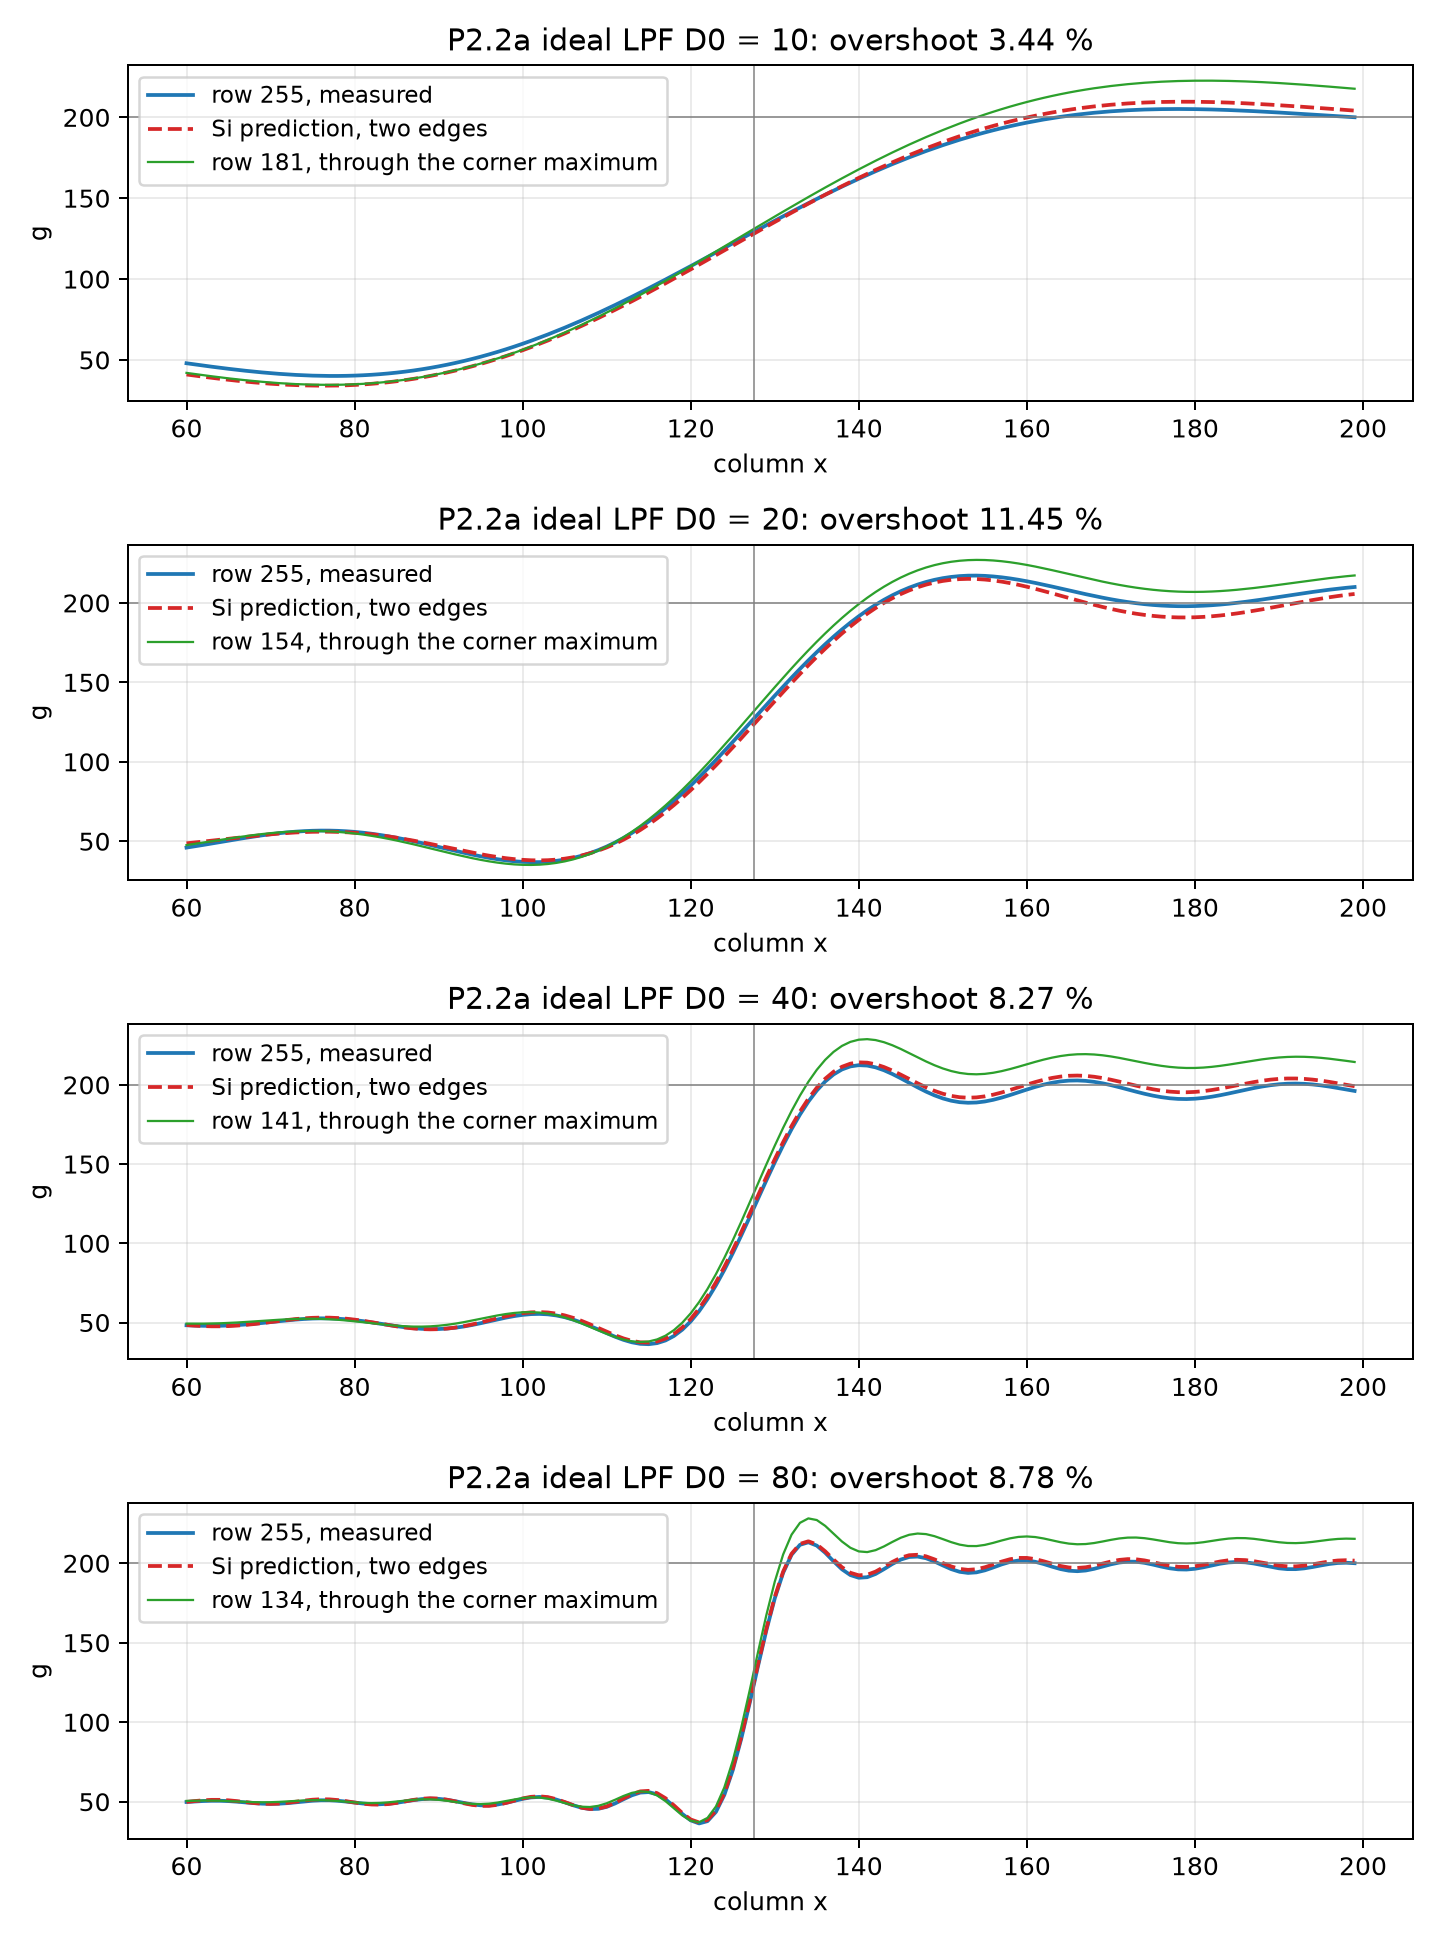
\includegraphics[width=0.95\linewidth]{problem_2/ideal_ringing_profiles.png}
\caption{Grey level against column: the measured row 255 (blue), the two-edge
prediction from \eqref{eq:si} (red, dashed) and the row through the corner
maximum (green), one panel per $D_0$.}
\label{fig:ringing}
\end{figure}

\paragraph{(b) Butterworth order sweep.} With $D_0=40$ the overshoot grows with
the order (Table~\ref{tab:bw}). The 1-D kernel $h(x)$ is the inverse DFT of the
central slice $H(u,0)$ of the $1024\times1024$ filter.

\begin{table}[H]
\centering
\begin{tabular}{lrrrrr}
\toprule
Filter & OS (\%) & $d$ (px) & $\min h$ & $\max h$ & $|\min h|/\max h$\\
\midrule
Butterworth $n=1$ & 0.0000 & none & $-2.938\times10^{-7}$ & $1.1663\times10^{-1}$ & $2.5191\times10^{-6}$\\
Butterworth $n=2$ & 3.3590 & 13.5 & $-3.749\times10^{-3}$ & $8.6763\times10^{-2}$ & $4.3207\times10^{-2}$\\
Butterworth $n=3$ & 5.6032 & 12.5 & $-7.906\times10^{-3}$ & $8.1812\times10^{-2}$ & $9.6639\times10^{-2}$\\
Butterworth $n=5$ & 7.4995 & 12.5 & $-1.253\times10^{-2}$ & $7.9425\times10^{-2}$ & $1.5775\times10^{-1}$\\
Butterworth $n=10$ & 8.4865 & 12.5 & $-1.569\times10^{-2}$ & $7.8447\times10^{-2}$ & $1.9995\times10^{-1}$\\
Butterworth $n=20$ & 8.4337 & 12.5 & $-1.661\times10^{-2}$ & $7.8205\times10^{-2}$ & $2.1236\times10^{-1}$\\
ideal & 8.2688 & 12.5 & $-1.719\times10^{-2}$ & $7.9102\times10^{-2}$ & $2.1730\times10^{-1}$\\
Gaussian $D_0=40$ & 0.0000 & none & $-1.388\times10^{-17}$ & $9.7915\times10^{-2}$ & $1.4\times10^{-16}$\\
Gaussian $D_0'=33.97$ & 0.0000 & none & $-6.939\times10^{-18}$ & $8.3161\times10^{-2}$ & $8.3\times10^{-17}$\\
\bottomrule
\end{tabular}
\caption{Overshoot and kernel ratio against Butterworth order, $D_0=40$,
$P=1024$. Every kernel sums to 1.00000.}
\label{tab:bw}
\end{table}

For $n=1$ the slice $1/(1+(u/D_0)^2)$ is a Lorentzian, and its inverse
transform is a two-sided exponential $\propto e^{-2\pi D_0|x|/P}$, which is
positive everywhere. The tiny minimum of $-2.9\times10^{-7}$ only comes from
cutting the slice off at $|u|=P/2$, and the overshoot is zero. For $n\ge2$ the
slice is flatter at the top and falls faster, and a transfer function that
falls faster than a Lorentzian needs negative lobes in its kernel. The ratio
$|\min h|/\max h$ rises from 0.043 at $n=2$ to 0.212 at $n=20$, close to the
ideal filter's 0.217, and the overshoot rises with it from 3.36\,\% towards the
ideal limit. The measured values for $n=10$ and 20 (8.49 and 8.43\,\%) sit a bit
above the measured ideal (8.27\,\%) because the same 2-D and other-edge effects
as in 2.2(a) act here too; the isolated-edge limit is 8.95\,\%.

\emph{Proof that a non-negative kernel cannot overshoot.} Let $h(k)\ge0$ with
$\sum_kh(k)=1$, and let the step $s$ only take values in $[A,B]$. The output
$g(x)=\sum_kh(k)\,s(x-k)$ is a weighted average of values of $s$ with
non-negative weights that add up to one, so
\[
A=\sum_kh(k)\,A\;\le\;g(x)\;\le\;\sum_kh(k)\,B=B\quad\text{for every }x.
\]
So $\max g\le B$ and the overshoot is at most zero. The same argument works in
2-D, so it covers the 2-D Butterworth filter with $n=1$ and the Gaussian, whose
kernels are positive. Ringing therefore needs negative lobes, and the kernel
ratio measures how big they are.

\paragraph{(c) Visual comparison.} Fig.~\ref{fig:grid} applies the three
families to the characters pattern at the four radii of Table~\ref{tab:power}.
At $r=15.3$ and 45.5 the ideal filter shows the ripples predicted above. The
insets in Fig.~\ref{fig:insets} mark two places: bright and dark bands parallel
to each side of the large black square, and light gaps between the vertical
bars that rise above the background level. Butterworth $n=2$ shows a faint
version of the same bands and the Gaussian shows none. Along the row through
the large square (\code{filter\_grid\_profile.png}) the ideal filter gives the
steepest edge. So at a given half-amplitude radius the trade-off is the one from
2.2(b): the sharper the transition in $H$, the sharper the edge and the stronger
the ringing. The Gaussian blurs the most and never rings, and Butterworth $n=2$
sits in between.

\begin{figure}[H]
\centering
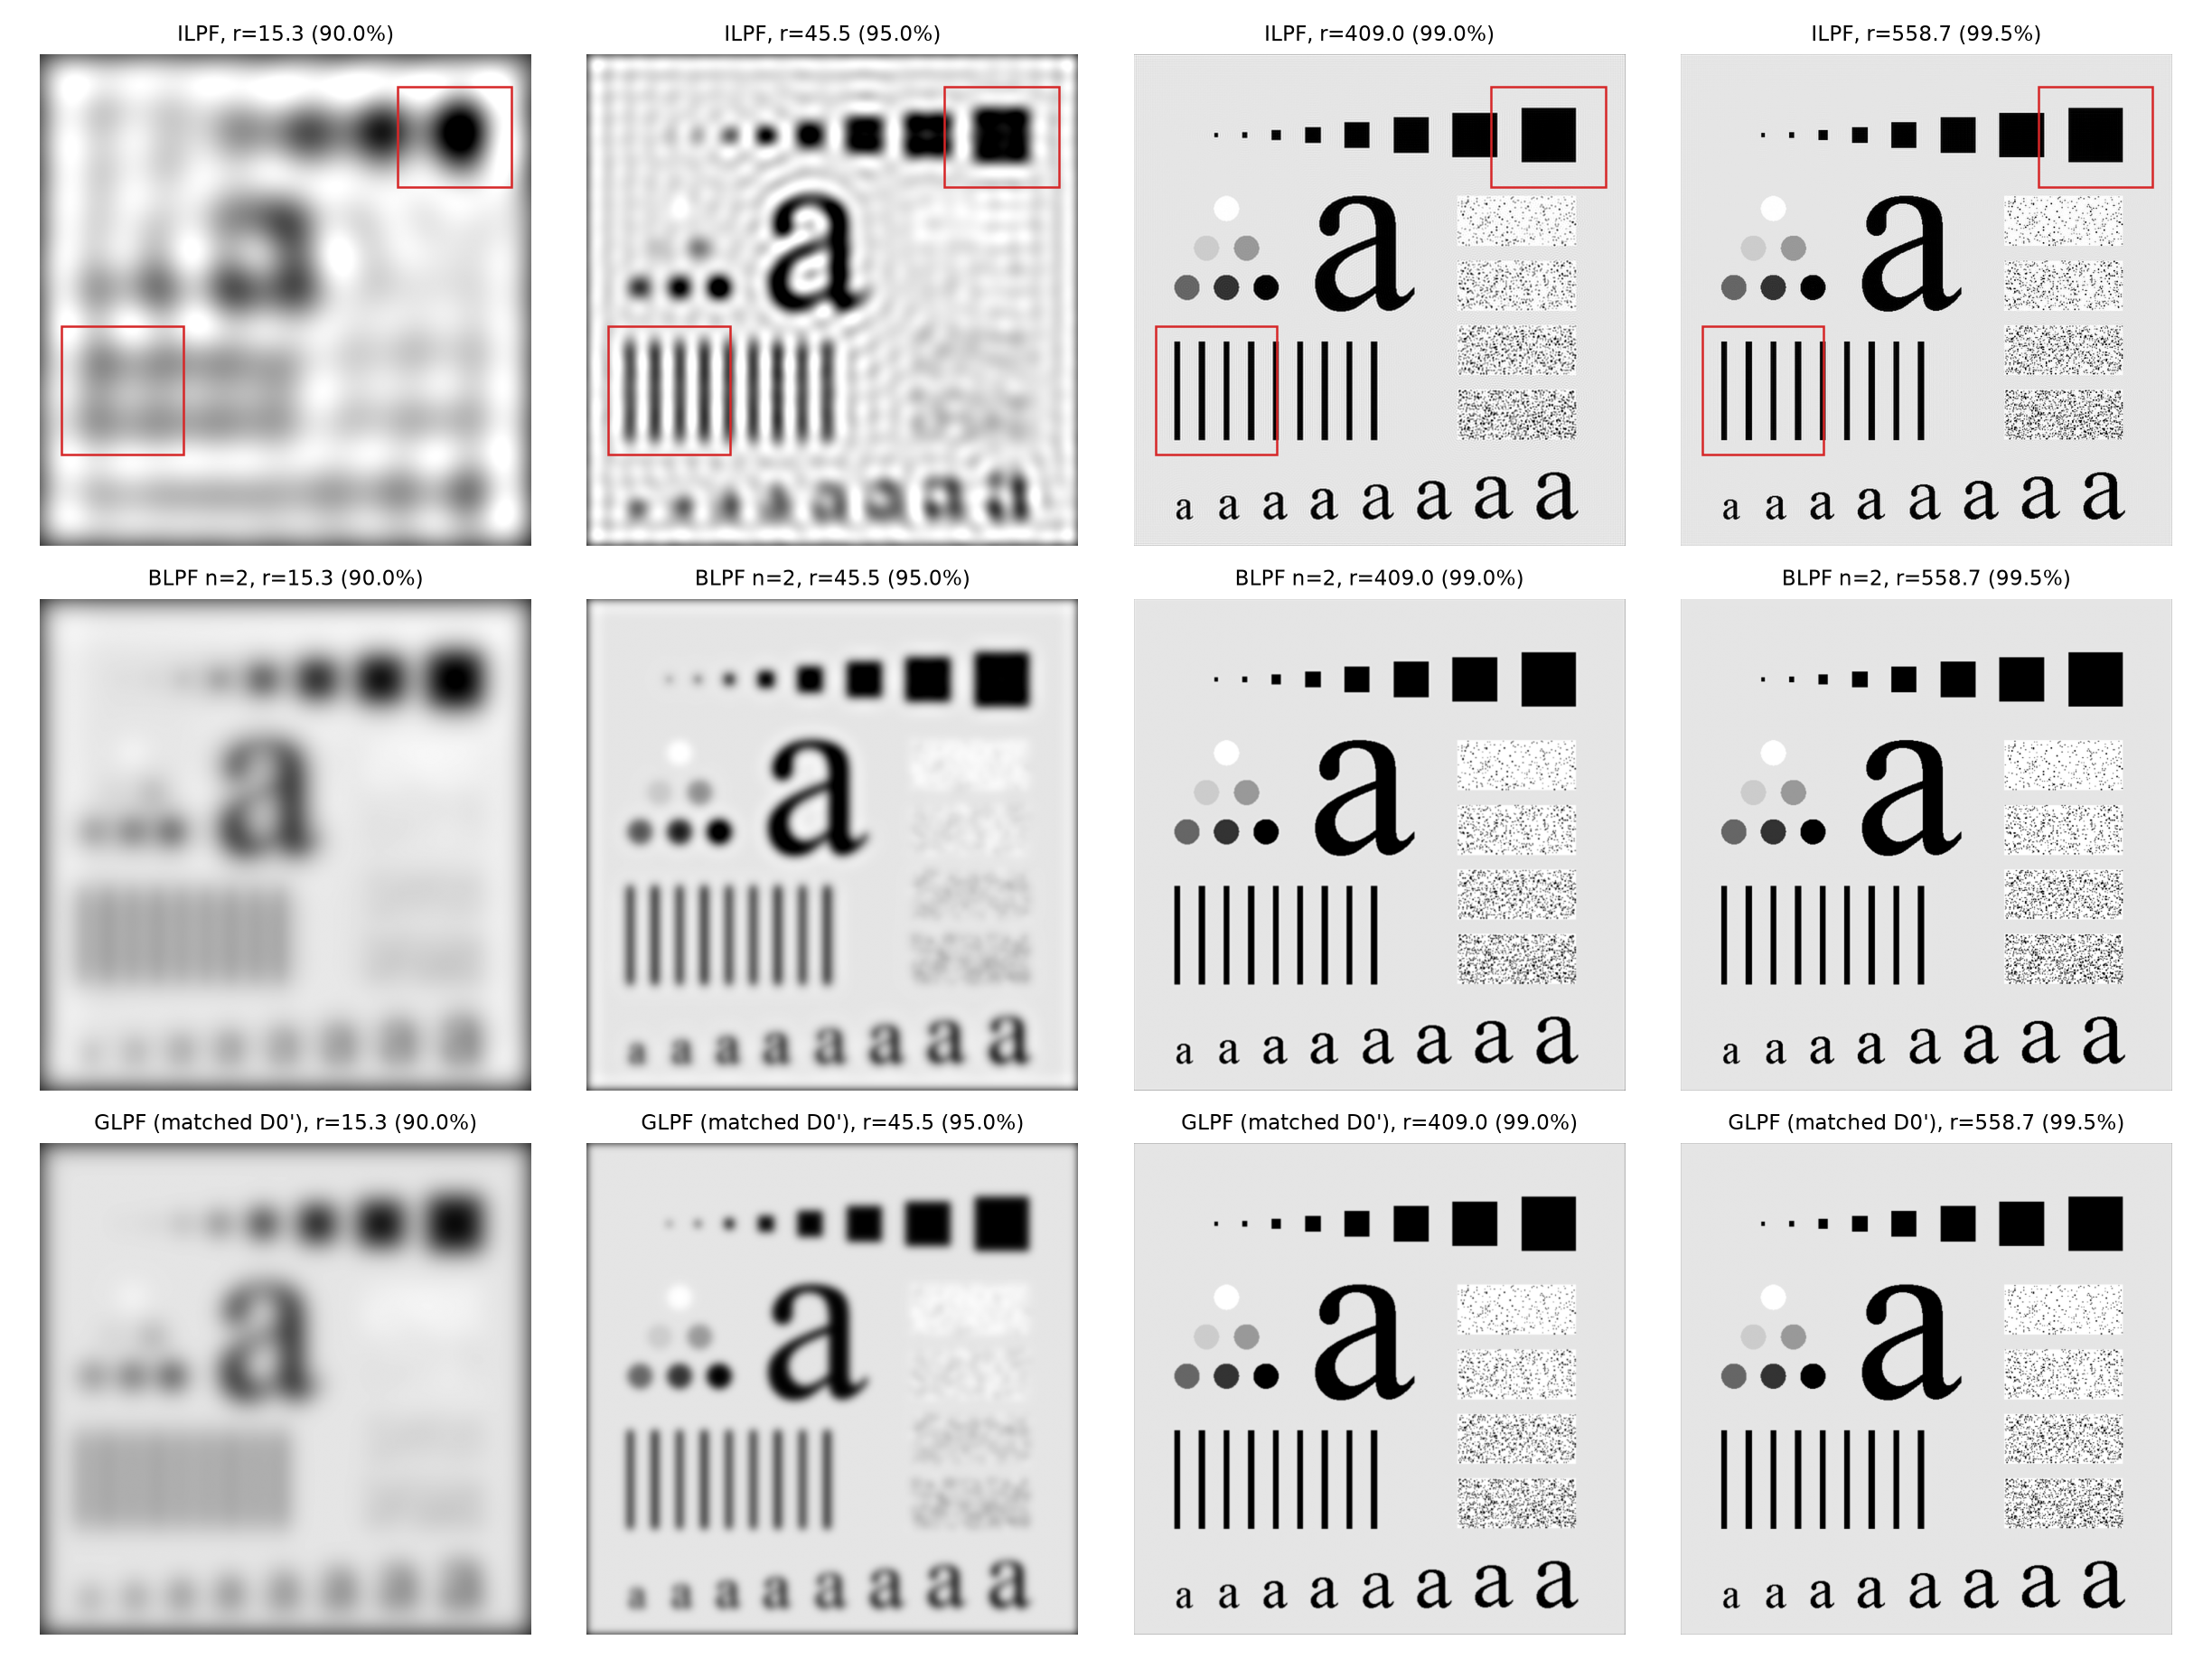
\includegraphics[width=\linewidth]{problem_2/filter_grid.png}
\caption{Rows: ILPF, BLPF $n=2$ and GLPF with the matched $D_0'$. Columns: the
radii that hold 90, 95, 99 and 99.5\,\% of the power. Red boxes mark the insets
of Fig.~\ref{fig:insets}.}
\label{fig:grid}
\end{figure}

\begin{figure}[H]
\centering
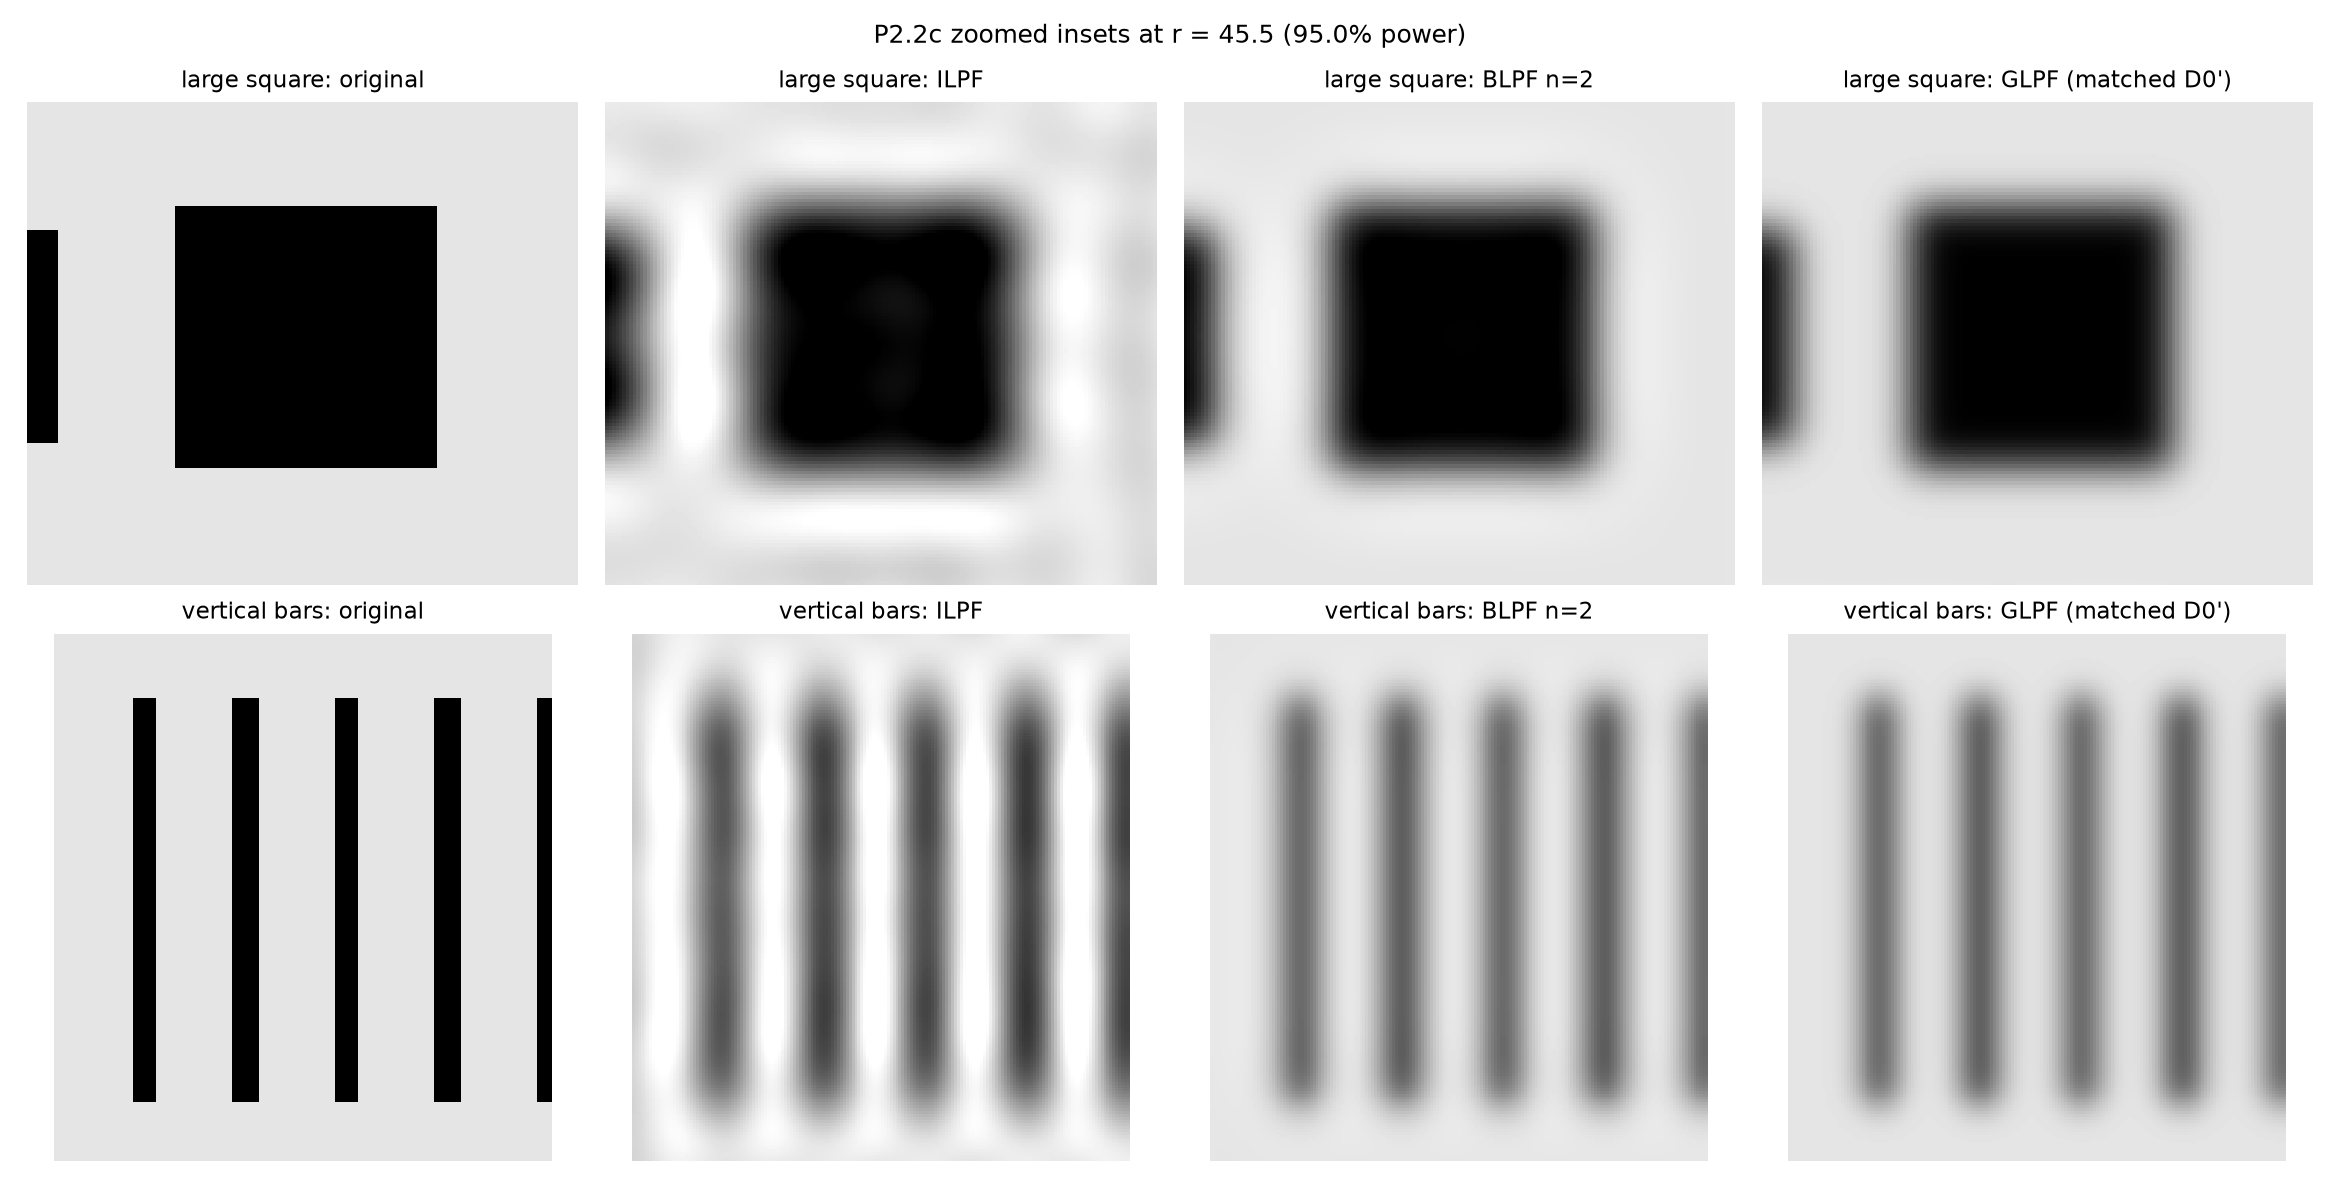
\includegraphics[width=0.9\linewidth]{problem_2/filter_grid_insets.png}
\caption{Ringing in the ideal low-pass output at $r=45.5$: bands beside the large
square and bright gaps between the bars.}
\label{fig:insets}
\end{figure}

\paragraph{(d) Gaussian equivalence.} The Gaussian slice is
$e^{-u^2/2D_0^2}$ with $u$ in bins, i.e.\ frequency $f=u/P$ cycles/pixel. A
spatial Gaussian of standard deviation $\sigma_s$ pixels has the transform
$e^{-2\pi^2\sigma_s^2f^2}=e^{-2\pi^2\sigma_s^2u^2/P^2}$. The two are equal when
$2\pi^2\sigma_s^2/P^2=1/(2D_0^2)$, so
\begin{equation}
\sigma_s=\frac{P}{2\pi D_0}.
\end{equation}
With $P=1376$ this is 21.90, 5.47 and 1.37 pixels for $D_0=10$, 40 and 160. I
ran SciPy's \code{gaussian\_filter} with this $\sigma_s$ and
\code{mode="constant"}, so its boundary matches the zero padding. This is the
comparison the handout asks for and the only place SciPy filters anything.

\begin{table}[H]
\centering
\begin{tabular}{rrrrrr}
\toprule
$D_0$ & $\sigma_s$ (px) & $H$ at $D=P/2$ & max error, truncate 4 & max error, truncate 8 & mean error, truncate 8\\
\midrule
10 & 21.8997 & 0 & $1.571\times10^{-2}$ & $6.253\times10^{-13}$ & $1.813\times10^{-13}$\\
40 & 5.4749 & $5.74\times10^{-65}$ & $1.766\times10^{-2}$ & $3.126\times10^{-13}$ & $5.015\times10^{-14}$\\
160 & 1.3687 & $9.66\times10^{-5}$ & $1.861\times10^{-2}$ & $3.306\times10^{-3}$ & $1.618\times10^{-4}$\\
\bottomrule
\end{tabular}
\caption{$\max|g_\text{freq}-g_\text{spatial}|$ in grey levels on the
characters pattern.}
\label{tab:gauss-eq}
\end{table}

There are two separate reasons the error is not zero. With SciPy's default
\code{truncate=4} the spatial kernel is cut at $4\sigma_s$ and renormalised,
which costs about $2\times10^{-2}$ grey levels at every $D_0$. With the kernel
extended to $8\sigma_s$, the agreement at $D_0=10$ and 40 is rounding, which
confirms the formula for $\sigma_s$. At $D_0=160$ an error of
$3.3\times10^{-3}$ is left, and this part grows with $D_0$ because of sampling.
The frequency-domain filter is a Gaussian that is cut off at the edge of the
$P\times P$ grid, where $H$ is still $9.7\times10^{-5}$. The spatial filter is a
Gaussian sampled at integer pixels, and the spectrum of a sampled function is
the continuous spectrum repeated at every integer frequency. When
$\sigma_s=1.37$ the kernel is barely two pixels wide, its spectrum is wide, the
repeated copies overlap near the Nyquist frequency, and the sharp edges of the
pattern have plenty of energy there. For wide spatial Gaussians (small $D_0$)
both effects disappear.

\subsection{Applications}

\paragraph{(a) Noise and blur.} I added zero-mean Gaussian noise with standard
deviation 20 (seed 2026, not clipped before filtering) to
\code{cameraman.tif}, which gives 22.459 dB. I swept each family over
$D_0=5,\dots,150$ in steps of 1, with $D_0$ the half-amplitude radius (the
Gaussian built with $D_0'$), and clipped the outputs to $[0,255]$ before
computing PSNR.

\begin{table}[H]
\centering
\begin{tabular}{lrrrrrr}
\toprule
Filter & best $D_0$ (5 to 150) & PSNR & best $D_0$ (all) & PSNR & PSNR, $D_0=30$ & PSNR, $D_0=100$\\
\midrule
ILPF & 150 & 27.491 & 215 & 28.690 & 19.723 & 24.940\\
BLPF $n=2$ & 150 & 28.735 & 210 & 29.719 & 20.418 & 26.219\\
GLPF (matched) & 150 & 28.517 & 215 & 29.558 & 20.324 & 26.107\\
\bottomrule
\end{tabular}
\caption{Low-pass denoising of \code{cameraman.tif}, $\sigma=20$, $P=1024$.
PSNR in dB, $D_0$ in bins.}
\label{tab:psnr-sweep}
\end{table}

\begin{figure}[H]
\centering
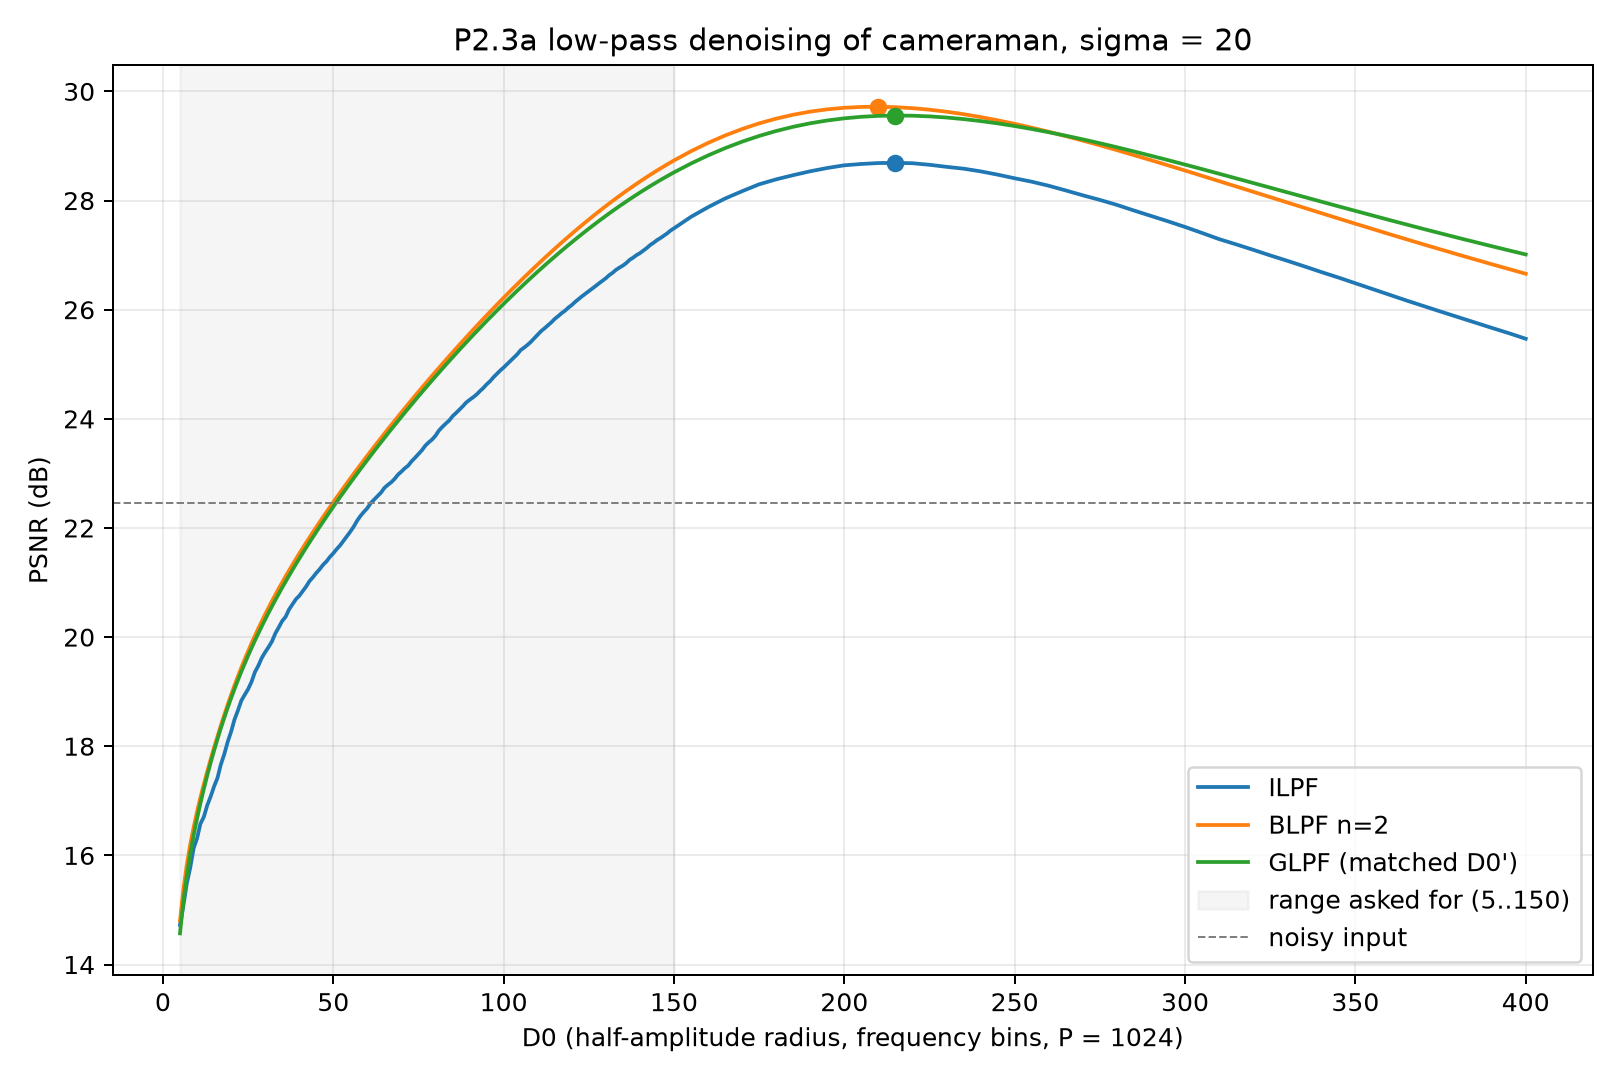
\includegraphics[width=0.7\linewidth]{problem_2/psnr_sweep.png}
\caption{PSNR (dB) against $D_0$ (bins on the $P=1024$ grid). The shaded band
is the range the handout asks for; I extended the sweep to 400 to find the
peaks.}
\label{fig:psnr-sweep}
\end{figure}

Inside the requested range all three curves are still rising at $D_0=150$, so
150 is the edge of the sweep and not an optimum. Extending the sweep in steps of
5 puts the real optima at 210 to 215. This is because of the padded grid:
$D_0=210$ on $P=1024$ is 0.205 cycles/pixel, the same frequency as
$D_0\approx105$ on the unpadded 512-point grid, where the optimum would fall
inside 5 to 150.

The curves peak where they do because white noise has the same power at every
frequency while the image's power falls steeply with frequency. Raising $D_0$
lets through more image detail but also more noise, and the best radius is
roughly where the image spectrum sinks to the noise level. The ideal filter has
the lowest peak (28.69 dB against 29.72 and 29.56 dB), and both reasons can be
read off its transfer function in Fig.~\ref{fig:tf}. It passes noise at full
gain right up to $D_0$ and removes all detail beyond it, whereas the smooth
filters let the noisy band fade out gradually. And its sinc kernel adds ringing
around every edge, which is extra error. The best Butterworth and Gaussian
results differ by only 0.16 dB, since at a matched half-amplitude radius their
transfer functions only differ in how steep the roll-off is. The best outputs
are in \code{psnr\_sweep\_best.png}.

\paragraph{(b) Character repair.} The text has 17766 dark pixels, and a
$3\times3$ morphological closing bridges 3602 gap pixels. I use those gap pixels
as a measurable stand-in for the broken strokes. Table~\ref{tab:text} gives, for
each Gaussian $D_0$, how dark the gaps become relative to the strokes
(``join''), how much darker the strokes stay than the background
(``contrast''), and how many 8-connected pieces are left after thresholding
halfway between the stroke and background levels. The pieces are counted with
my own union-find labelling (\code{label\_components} in
\code{src/common/metrics.py}), which the unit tests check against
\code{scipy.ndimage.label}.

\begin{table}[H]
\centering
\begin{tabular}{rrrrrr}
\toprule
$D_0$ & stroke & gap & join & contrast & pieces\\
\midrule
original & 1.000 & 0.000 & 0.000 & 1.000 & 266\\
40 & 0.292 & 0.273 & 0.933 & 0.274 & 43\\
60 & 0.364 & 0.342 & 0.940 & 0.357 & 102\\
70 & 0.399 & 0.371 & 0.930 & 0.396 & 169\\
\textbf{80} & \textbf{0.433} & \textbf{0.396} & \textbf{0.913} & \textbf{0.431} & \textbf{191}\\
90 & 0.465 & 0.415 & 0.893 & 0.464 & 196\\
120 & 0.548 & 0.448 & 0.819 & 0.548 & 201\\
200 & 0.698 & 0.417 & 0.598 & 0.698 & 208\\
\bottomrule
\end{tabular}
\caption{Gaussian repair of \code{text\_gaps}, $P=1016$ (selected rows of
\code{text\_repair.txt}). Stroke, gap and contrast are darkness
$(255-g)/255$.}
\label{tab:text}
\end{table}

I chose $D_0$ with a written rule: the gaps must be at least 90\,\% as dark as
the strokes, and at most 10\,\% of the pieces may be lost to letters merging,
compared with the least blurred setting (208 pieces at $D_0=200$). I wrote the
rule after a first look at this table, so it states my visual choice precisely
rather than being independent of it. Only $D_0=80$ meets both conditions. Below
it, letters start to fuse (169 pieces at 70, 43 at 40); above it, the gaps stay
visibly lighter than the strokes. In Fig.~\ref{fig:text} the strokes are joined
and the text reads easily.

An ideal filter with the same half-amplitude radius ($80\sqrt{2\ln2}=94.19$)
joins the gaps even more strongly (join 0.977), but its sinc kernel rings. The
output ranges from 37.9 to 317.6 on a 0 to 255 image, every character gets
light and dark halos, and the halos link neighbouring letters, so only 83
pieces are left.

\begin{figure}[H]
\centering
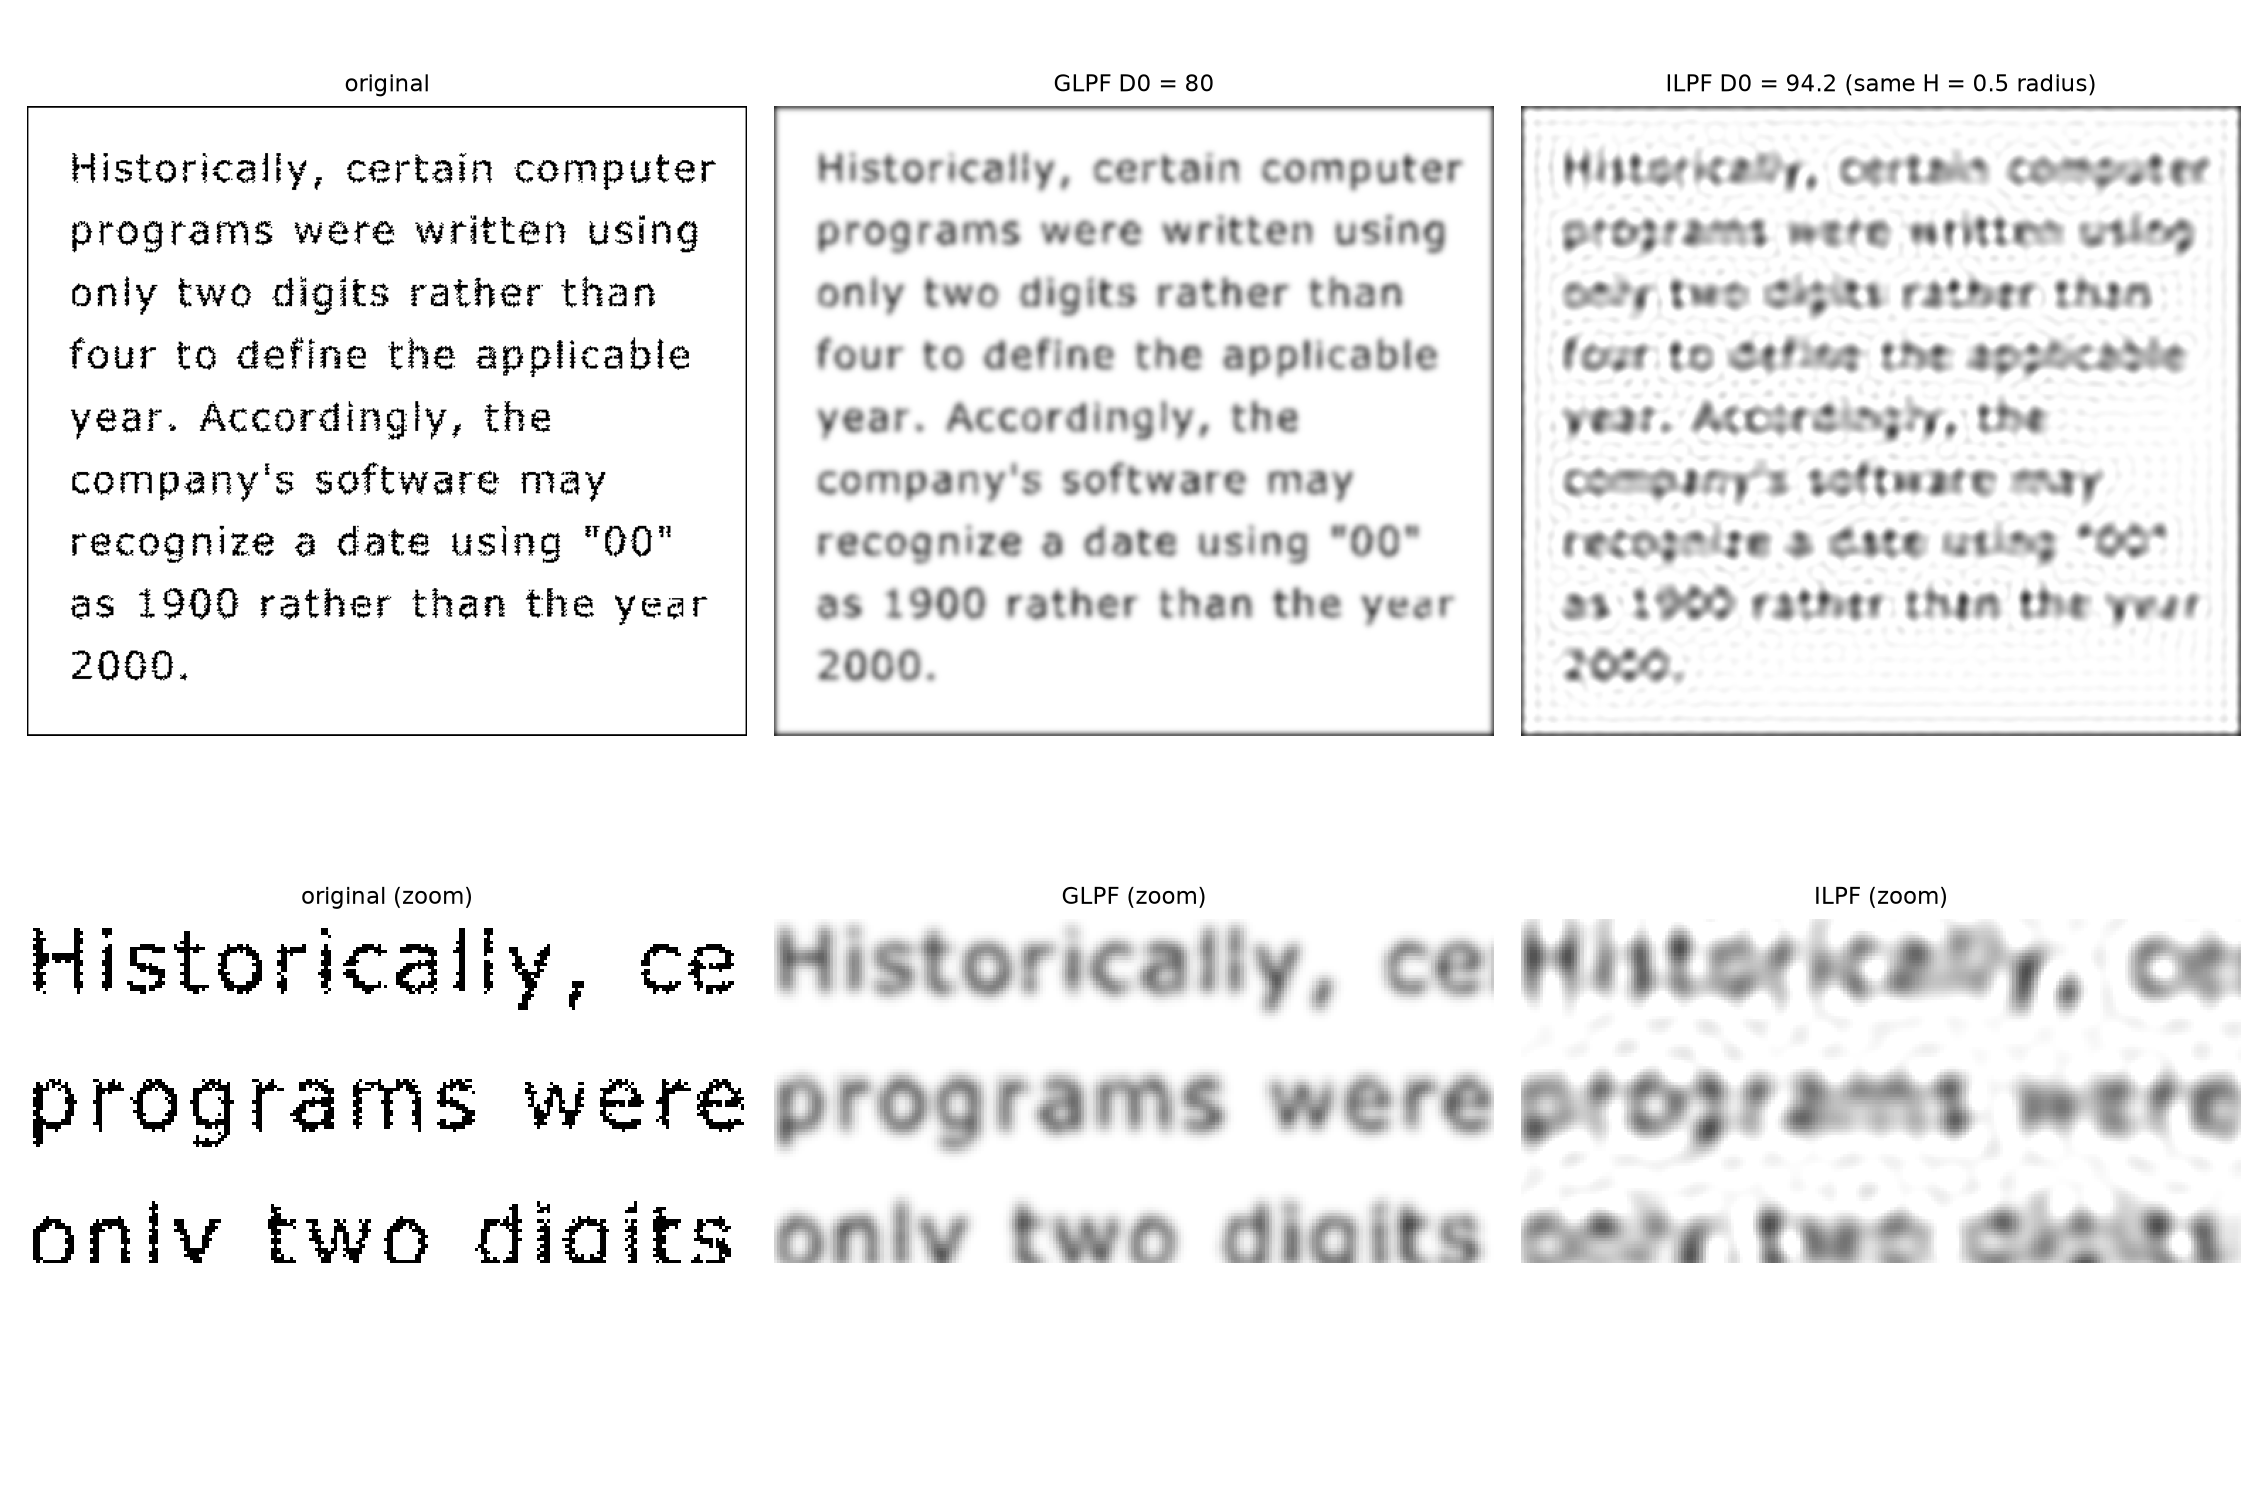
\includegraphics[width=0.85\linewidth]{problem_2/text_repair.png}
\caption{Original, Gaussian $D_0=80$, and the ideal filter with the same
half-amplitude radius, with zoomed crops below.}
\label{fig:text}
\end{figure}

\paragraph{(c) High-pass, DC and emphasis.} I filtered \code{thumb\_print.tif}
with IHPF, BHPF $n=4$ and GHPF at a common half-amplitude radius of 50
($P=2052$).

\begin{table}[H]
\centering
\begin{tabular}{lrrrrrr}
\toprule
Filter & $H_\text{HP}(P/2,P/2)$ & mean (crop) & mean ($P\times P$) & std & pieces $>0$ & specks $<20$ px\\
\midrule
IHPF & 0 & 1.4226 & $8.29\times10^{-17}$ & 32.032 & 840 & 767\\
BHPF $n=4$ & 0 & 1.4588 & $4.15\times10^{-17}$ & 31.486 & 868 & 790\\
GHPF & 0 & 2.0654 & $5.53\times10^{-17}$ & 30.400 & 1088 & 991\\
\bottomrule
\end{tabular}
\caption{High-pass outputs (input mean 142.728). ``Pieces'' and ``specks''
count the 8-connected regions of the ridge map $g>0$.}
\label{tab:hp}
\end{table}

All three filters have $H_\text{HP}(P/2,P/2)=1-H_\text{LP}(0)=0$. The centre
bin is the DC term, which equals $P^2$ times the mean, so the filter removes it
and the mean of the full padded output is zero up to rounding. The mean over the
cropped image is not exactly zero (1.4 to 2.1) because the zero-mean property
holds for the whole $P\times P$ array, and the filtered jump from the image to
the zero padding leaves negative values outside the crop. Compared with the
input mean of 142.7, the tonal information is gone, which is why the high-pass
images look mid-grey.

High-frequency emphasis $H_\text{HFE}=k_1+k_2H_\text{HP}$ with $k_1=0.5$ and
$k_2=0.75$ (Gaussian $H_\text{HP}$) keeps half of the DC and low frequencies and
multiplies the high frequencies by $k_1+k_2=1.25$. Ridges therefore gain a
factor of 2.5 relative to the slow shading, while the tones survive. The output
mean is 72.913, close to $k_1\cdot142.728=71.364$ (the rest is again the crop
effect). The overall spread stays the same as the input's (standard deviation
40.455 against 40.427), but it is redistributed: the shading across the print is
halved and the ridges are sharper (Fig.~\ref{fig:hp}).

Thresholding each high-pass output at zero gives a ridge map. By the number of
small specks, the ideal (767) and Butterworth (790) maps are about equally clean
and the Gaussian map is clearly the noisiest (991). At a common half-amplitude
radius the Gaussian high-pass rises slowly: at $D=25$ it already passes 16\,\%
of the low frequencies, against 0.4\,\% for Butterworth $n=4$ and 0 for the
ideal filter. That leaked shading moves the zero crossings and breaks ridges
into fragments. The ideal and Butterworth maps both show a dark band along the
top border, where the print meets the zero padding and the filter responds to
that artificial edge. Butterworth $n=4$ has almost the steep roll-off of the
ideal filter without its sinc kernel, so it is the safer choice, although on this
image the speck count does not separate the two.

\begin{figure}[H]
\centering
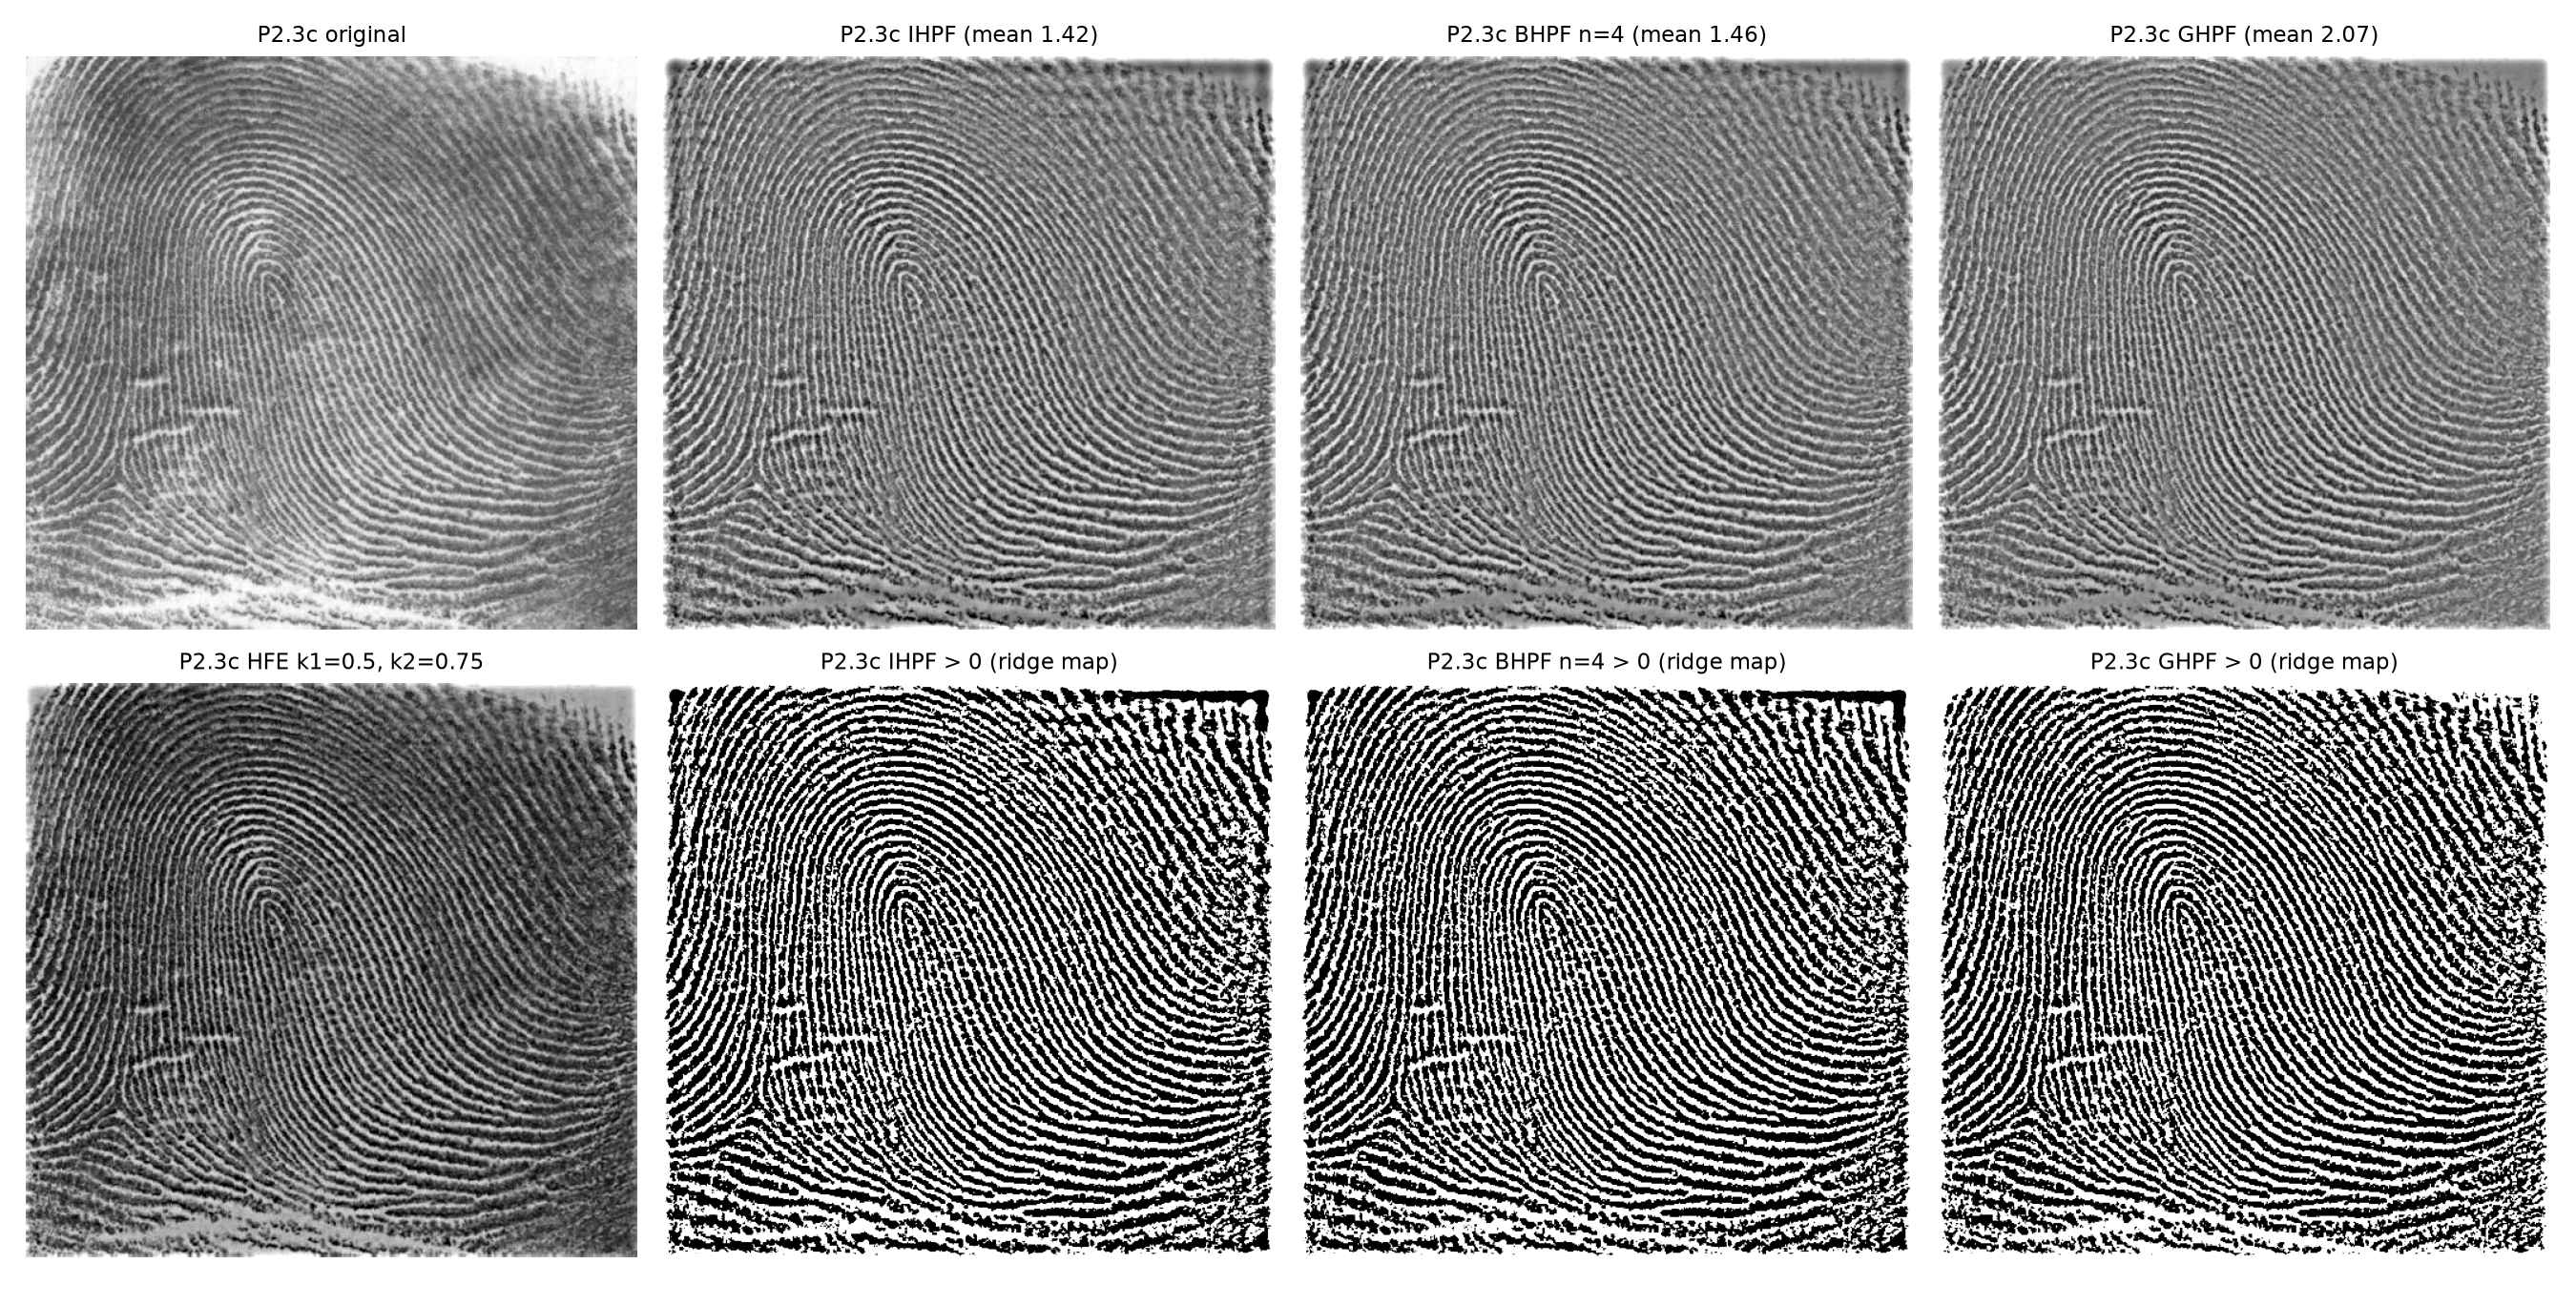
\includegraphics[width=\linewidth]{problem_2/highpass.png}
\caption{High-pass outputs (on a symmetric grey range), high-frequency emphasis,
and the ridge maps from thresholding at zero.}
\label{fig:hp}
\end{figure}
